% TikZ 2D: geometric shapes with fills, borders, and labels
\documentclass{article}
\usepackage{tikz}
\usetikzlibrary{patterns, shapes.geometric}

\begin{document}
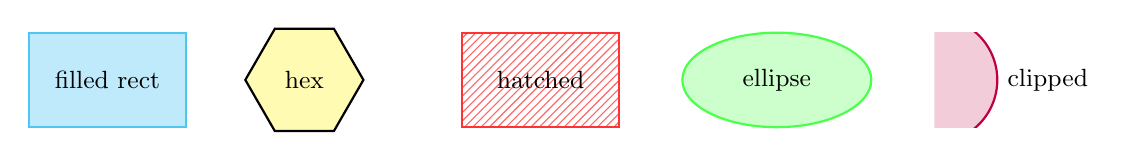
\begin{tikzpicture}[font=\small, line width=0.8pt]

  % Filled + stroked rectangle
  \filldraw[fill=cyan!25, draw=cyan!70]
    (0,0) rectangle (2,1.2);
  \node at (1,0.6) {filled rect};

  % Regular polygon (hexagon)
  \node[draw, fill=yellow!30, regular polygon, regular polygon sides=6,
        minimum size=1.5cm] at (3.5,0.6) {hex};

  % Hatched region (patterns library)
  \fill[pattern=north east lines, pattern color=red!60]
    (5.5,0) rectangle (7.5,1.2);
  \draw[red!80] (5.5,0) rectangle (7.5,1.2);
  \node at (6.5,0.6) {hatched};

  % Ellipse
  \filldraw[fill=green!20, draw=green!70]
    (9.5,0.6) ellipse (1.2 and 0.6);
  \node at (9.5,0.6) {ellipse};

  % Clipped circle (only show right half)
  \begin{scope}
    \clip (11.5,0) rectangle (13.5,1.2);
    \filldraw[fill=purple!20, draw=purple]
      (11.5,0.6) circle (0.8);
  \end{scope}
  \node[right] at (12.3,0.6) {clipped};

\end{tikzpicture}
\end{document}
